%%
\chapter{Generating query based monitoring components}
%%

Before the monitoring components can be generated and deployed, we must design the system. First, the metamodel must be designed, and after the metamodel is specified, we define graph queries, as they depend on the metamodel of the graph on which they are evaluated. As stated before, these two steps are done using EMF and \viatra{} technologies.

In this chapter, I present how the monitoring components are generated from this these artifacts. 

\section{Generating classes from the metamodel}

The types of the metamodel are mapped to \cpp{} classes in the following way: From each type we generate three \cpp{} classes:

\begin{enumerate}
	\item An interface which provides access to an object of the type
	\item A local class, that stores the attributes and references of the instances allocated to the local computing unit.
	\item A proxy class, which can be used to substitute remote objects in references to them.
\end{enumerate}


\section{Overview of the query compilation workflow}

The compilation of the queries of the CPS is depicted in fig. \ref{figure:query-compile-workflow}. First, the local search planner of the \viatra{} system creates a plan. We complete the generated plan with types and other supplementary information and make a distributed version of the plans. After that, we use additional optimization specialized for our execution mechanism to improve the execution. After the fully optimized plan is ready, we can construct the generator model describing the source code structure and generate the \cpp{} files.

\begin{figure}[h]
	\begin{center}
		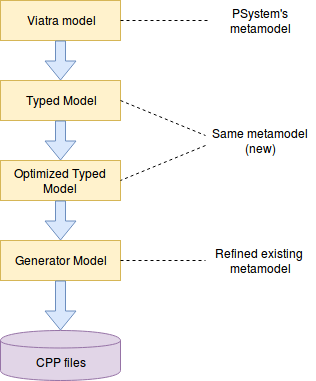
\includegraphics[width=0.5\textwidth]{figures/workflow.png}
		\caption{Query comompilation workflow}
		\label{figure:query-compile-workflow}
	\end{center}
\end{figure}


\section{Viatra plan}

The query file is processed by \viatra{}~\cite{viatra} and a local search plan is generated. In case of local search, the plan is a sequence of search operation defined as an application of a constraint.


\section{Completed plan}

\viatra{} generated plans are not intended for external usage. We need to complete it with additional information to use it for our purposes. One of the main concern is type information. To obtain type information we use the constraints to deduce the type of a variable. 


\section{Additional optimization}

After we complete the plan with type information and other details, it can be used to generate C++ code, although before that step we use further optimizations. These optimizations considers distributed execution of the plan, so it can improve the plan generated by \viatra{} which is generated to be used in a single computer.


\subsection{Replace pattern calls with simpler operations}
There are some cases, where helper patterns are simple, and used to define simple conditions. In this case, evaluationg the subquery is not always the most efficient method, sometimes these can be replaced by simple search operations:

\subsubsection{Reference Pattern}
We use the phrase \emph{reference pattern} for a pattern with 2 parameters if its only constraint is that a reference exist between the two parameters, eq.:
\begin{lstlisting}[language = vql]
private pattern connected(a : RailRoadElement, b : RailRoadElement){
	RailRoadElement.connectedTo(a,b);
}
\end{lstlisting}
In the following examples i will use this query as an example to demonstrate how the application of this query can be replaced by an other operation.

\subsubsection{Counting reference pattern}
\subsubsection{Negative application of a reference pattern}

\subsection{Filter unnecessary operations, checks}
As the original plan is generated by the localsearch planner of \viatra{}, there can be redundant operations, which can be ommited. This includes:

\begin{itemize}
	\item Check operation -- The generated code is strongly typed, so we don't need type checks in most cases, unlike in the Java implementation, where the tuples contains plain java objects with unknown types.
	
	\item Distribution operations -- \todo{KIFEJTENI}
\end{itemize}



\section{C++ code generation}

The completed and optimized plan are used to generate \cpp{} code. Two main methods can be used to run local search plan in case of generated code. One is to generate the plan as a data structure and create an interpreter that uses that plan to find matches. The other is to generate the code directly from the plan. The first method is good if we want to change the plan at runtime, but the interpreter itself introduces an overhead, causing performance to be slower. We used the later, because we don't change the plan at runtime.












